\chapter{Introduction}

This document is intended to describe the main steps required for the integration and configuration of \LongName module.
%\ifnum \DocumentGroup=1
%{
%General guidelines on the common steps and workflow for RTA-SUM integration can be found in RTA-SUM Getting Started Guide.
%}
%\else
%{
%Nothing
%}\fi

\section{Definitions and Abbreviations}
\input{generated/tables/definitions.tex}

\section{Module Overview}
The RTA-SUM TCS, Global Time Client Service, is a software composition located in
the Application Layer of the standardized architecture of AUTOSAR.


TCS is primarily intended to be used to provide a synchronized time stamp for the extended date
record of a DTC. It fulfills the requirements of a TS Slave per the "SDV-6001 ECU Diagnostic
Infrastructure Requirements" specification and is not intended to provide any control functions
or vehicle driver / passenger viewable display data.


TCS receives a signal (TimeSyncMessage) via the serial data communication bus from an ECU
which has the Master Clock function. The resolution and transmission rate of the Master Clock signal is
as defined by the diagnostic team.


TCS is responsible for the following functions:
\begin{itemize}
\item Receive the global time from the Master Clock global time provider via serial data
communication
\item Synchronize the local ECU time to the master global time
\item Substitute the last received value (default if never received) following initialization, until the
initial Master Clock signal is received via serial communication
\item Keep a local timer source to maintain ECU internal time source between reception events of the Master Clock signal.
\item Provide a DID Interface to the diagnostic module DCM, providing current timing client local time value.
\end{itemize}

TCS shall take appropriate actions in response to the above functions, such as:


\begin{itemize}
\item Correction to locally computed time each time the master global time signal is received
\item Update time (locally) for periods when the Master Clock global time signal cannot be received because no Partial Network on a communication channel is not active. (Master Clock is expected to be part of all PNs)
\item Provide unique Time Synch signal to Dem based on Master Clock global time signal.
\end{itemize}

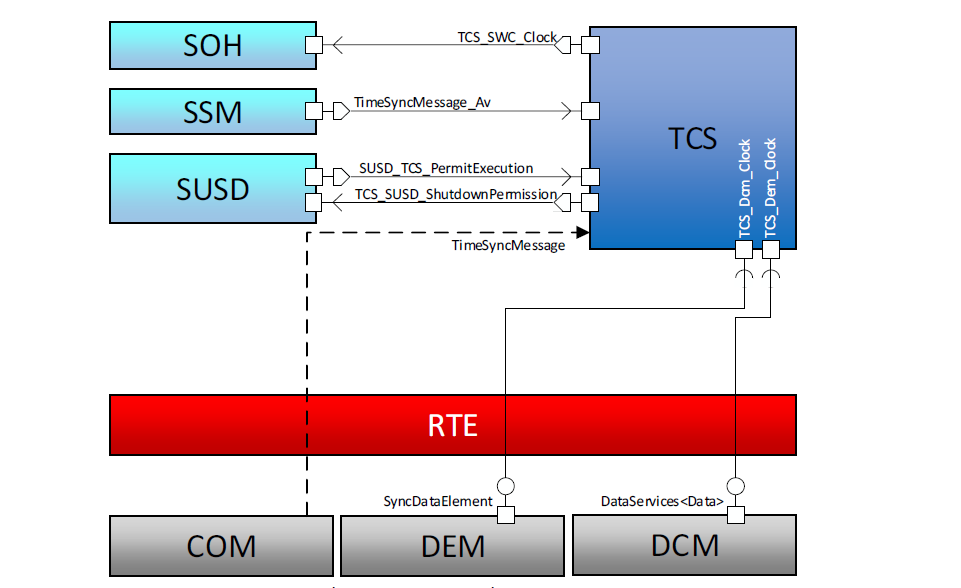
\includegraphics[scale=0.7]{images/block.png}

\section{References}
\input{generated/tables/references.tex}

\section{User Guide Revision History}
\input{generated/tables/rev_history.tex}